\chapter{Implementation}

This section will focus upon the implementation of the various artefacts, in 
order to successfully create the software product associated with this project.

All code artefacts will be expressed in pseudocode, with an implementation of 
the code snippet available upon the supplied CD-ROM. 

% C# Style
\definecolor{bluekeywords}{rgb}{0.13,0.13,1}
\definecolor{greencomments}{rgb}{0,0.5,0}
\definecolor{redstrings}{rgb}{0.9,0,0}

\lstdefinestyle{csharp}{
  language=[Sharp]C,
  showspaces=false,
  showtabs=false,
  breaklines=true,
  showstringspaces=false,
  breakatwhitespace=true,
  escapeinside={(*@}{@*)},
  commentstyle=\color{greencomments},
  keywordstyle=\color{bluekeywords}\bfseries,
  stringstyle=\color{redstrings},
  basicstyle=\ttfamily
}

 
\lstdefinestyle{pseudocode}{
  language=C,
  showspaces=false,
  showtabs=false,
  breaklines=true,
  showstringspaces=false,
  breakatwhitespace=true,
  commentstyle=\color{greencomments},
  keywordstyle=\color{bluekeywords}\bfseries,
  stringstyle=\color{redstrings},
  basicstyle=\footnotesize\ttfamily,
  morekeywords={WHILE, END, READ, CREATE, IF, NOT, DO, ELSE, FOR, WRITE, ADD,
                COMPRESS, RENAME, REMOVE, SAVE, REPEAT, UNTIL, SET, RETURN,
                CONVERT}
}


% KML File Handling
\newpage
\section{KML File Handling}

As previously mentioned figure \ref{fig:NSKML} illustrates the namespace that 
handles the reading of KML files and writing of KML and KMZ files. Within this 
section the implementation of these classes will be discussed.

\subsection{KML Reader}
The KML Reader class encapsulates an {\ttfamily XmlTextReader} object for 
which the class can be found within the {\ttfamily System.Xml} namespace. 

A KML file is a well formed XML file, and hence the reason why the 
{\ttfamily XMLTextReader} class was able to be used for the majority of the 
parsing procedure.

The main method within the file is the {\ttfamily GetCallLogs()} method, which
will return an event collection of events from the given KML file. 

If an invalid KML file is found, or no placemarks are able to be fully 
retrieved from the KML file, then the method will simply return an empty Event 
collection.

~\\
{\bfseries KMLReader::GetCallLogs()}
\lstset{style=pseudocode}
\begin{lstlisting}
  WHILE not at the end of the file
    // Obtain the Coordinate information
    READ the coordinate tag

    // Obtain the additional meta-data
    READ the device name tag
    READ the device pin tag
    READ the timestamp tag
    READ the reference tag
    READ the type tag
    READ the start rat tag
    READ the end rat tag
    READ the start mix band tag
    READ the end mix band tag
    READ the start rrc state tag

    // Create a new Event based upon the above information
    CREATE a new Event based upon the coordiante and meta-data

    // Add the parsed event
    ADD the event to the List of Events
  END WHILE

  RETURN List of Events
\end{lstlisting}
{\textsf \footnotesize File Source: src/KML/KMLReader.cs }

\subsection{KML Writer}
The KML Writer class encapsulates an {\ttfamily XmlTextWriter} object, for 
which the class can be found within the the {\ttfamily System.Xml} namespace. 

As previously mentioned, a KML file is a well formed XML file, and 
{\ttfamily XmlTextWriter} object can be used to generate a well formed KML 
file.

The main entry point for the KMLWriter class is the {\ttfamily GenerateKML()} 
method. This method is able to take a number of parameters in order to generate
a well formed KML file, and is able to perform multiple options based upon the 
given parameters.

~\\
{\bfseries KMLWriter::GenerateKML()}
\lstset{style=pseudocode}
\begin{lstlisting}
  // Create a new KML file at a given location
  CREATE new kml file

  // Insert the heatmap if given
  IF heatmap present
    ADD heatmap reference to the kml file
  END IF

  // Loop over each cluster
  FOR each cluster in clusters
    // Organise events into their clusters
    WRITE a new cluster folder

    // Loop over each event in the cluster
    FOR each event in cluster
      WRITE event to the cluster folder
    END FOR

  END FOR

  // Write noise data if available
  IF noise present
    // Organise noise events into a noise folder
    WRITE a new cluster folder

    // Loop over each noisy event
    FOR each event in noise
      WRITE event to the noise cluster folder
    END FOR

  END IF
\end{lstlisting}
{\textsf \footnotesize File Source: src/KML/KMLWriter.cs }


\subsection{KMZ Writer}
A KMZ file is a compressed KML file. One the advantages of using a KMZ file 
over a KML file is that the file is able to store images embedded directly in
itself. This is unlike a KML file, where by an image must be referenced.

The KMZWriter class has a dependency upon the KMLWriter class. The main entry 
point to the KMZWriter class is through the {\ttfamily GenerateKMZ()} method.

The method will utilise the KMLWriter class to create the KML file, and will 
then place all generated files into a compressed KMZ file.

~\\
{\bfseries KMZWriter::GenerateKMZ()}
\lstset{style=pseudocode}
\begin{lstlisting}
  // Create a new temporary working directory
  CREATE new temporary directory

  // This will create a new KML file.
  // A heatmap may also be created
  CREATE kml file and SAVE into the temporary

  // Create the temporary archive
  COMPRESS the temporary directory into an archive

  // Forms the KMZ file
  RENAME the archive extension to .KMZ

  // Remove all working files and folders
  REMOVE the temporary directory
\end{lstlisting}
{\textsf \footnotesize File Source: src/KML/KMZWriter.cs }


% Clustering - DBSCAN
\newpage
\section{DBSCAN}

The DBSCAN class provides an interface to allow for clustering of a collection 
of events. The formal description of the DBSCAN methodology and algorithm can 
be found within section \ref{sec:DBSCAN}.

For reference purposes, the basic DBSCAN algorithm is outlined below:
\begin{enumerate}
  \item Label all points as core or noise points;
  \item Eliminate noise points;
  \item Put an edge between all core points that are within {\em Eps} of each 
        other;
  \item Make each group of connected core points into a separate cluster;
  \item Assign each border point to one of the clusters of its associated core 
        points.
\end{enumerate}


\subsection{Analyse Data}
The main entry point to start the algorithm is through the use of the 
{\ttfamily Analyse()} method. The algorithm will automatically determine if 
points are noise, and if noise points are found they are removed from the 
results.

There is no limit to the number of clusters that can be generated, however 
there is a minimum number of points that are required to form a cluster. This 
value is represented by the minPts value.

~\\
{\bfseries DBSCAN::Analyse()}
\lstset{style=pseudocode}
\begin{lstlisting}
  // The "current working" cluster
  cluster = null;

  // Loop over all unvisisted events
  FOR each unvisisted event (E) in the dataset (D)
    // Prevent a revisit of the current event
    SET E as visited

    // Obtain all neighbourhood events 
    NeighbourhoodEvents = all events within the EPS distance of E

    // Ensure that there are sufficent events
    IF the total amount of NeighbourhoodEvents < MinimumPoints
      SET E as NOISE
    else
      C = next cluster
      expand all the Neighbourhood events to determine similarity
    END IF

  END FOR
\end{lstlisting}
{\textsf \footnotesize File Source: src/Clusters/DBSCAN.cs }


\subsection{Neighbourhood Search}
The {\ttfamily GetRegion()} method will return all events that are within the 
eps-neighbourhood of a given event.

~\\
{\bfseries DBSCAN::GetRegion()}
\lstset{style=pseudocode}
\begin{lstlisting}
  // The "central", given event
  Evt = given event
  
  // Loop over all known events
  FOR each event (E) in dataset (D)

    // Calculate the distance between the events
    distance = distance from E to Evt

    // Add the event if it's deemed to be a neighbour
    IF eps >= distance
      ADD E to neighbours

  END FOR
\end{lstlisting}
{\textsf \footnotesize File Source: src/Clusters/DBSCAN.cs }


\subsection{Expanding a Cluster}
The {\ttfamily ExpandCluster()} method will expand each of the event 
neighbours, and all of their neighbours. 

Ultimately, this method will deduce which events are within the given event's 
EPS neighbourhood, and hence whether or not they belong to a new cluster.

~\\
{\bfseries DBSCAN::ExpandCluster()}
\lstset{style=pseudocode}
\begin{lstlisting}
  // The given event
  GivenEvt = given event

  // Add the current event to a new cluster
  ADD event to cluster (C)

  // Get the all of evt's neighbours.
  neighbours = get all events within GivenEvts region

  // Loop over each event in GivenEvt's neighbours
  FOR each event evt in neighbours

    // Visit the evt if it has not been visited
    if evt has not been visited

      // Mark as visited
      SET evt as visited
      
      // Obtain all the events within the new region
      evtNeighbours = get all events within evts region

      // Assume all are non-noise if greater than the MinimumPoints value
      IF the total amount of NeighbourhoodEvents >= MinimumPoints

        // Merge the two neighbours lists together
        ADD evtNeighbours onto the end of neighbours
      END IF

    END IF

    // If the event doesn't belong to a cluster add to a new cluster
    IF evt does not belong to a cluster

      // Add the event to the cluster
      add evt to C
    END IF

  END FOR
\end{lstlisting}
{\textsf \footnotesize File Source: src/Clusters/DBSCAN.cs }

% Analysis
\newpage
\section{Analysis}
The Analysis aspect of the project is split up across two libraries --- 
Analysis and Analysis.Heatmap.

The first library focuses upon providing analysis for clusters on a product 
level and a week level. The library also supports multi-product and multi-week 
analysis.

The second library focuses upon providing support for generating a heatmap from
a given set of events. The library is able to change the colour scheme of the 
generated heatmap if required to.


\subsection{Analysis}
The EventAnalysis class forms the basis of all types of analysis --- referred 
to as primary analysis. The primary analysis defines operations such as the 
number of events that happened within a given cluster.

The analysis also tries to group similar events together to further highlight 
any similarities (or differences) within an intra-cluster environment, and 
across multiple weeks.

The {\ttfamily GetRatCount()} and {\ttfamily GetMixBandCount()} methods will 
return the number of events that started upon the a given RAT or MixBand 
respectfully.

Only one of the methods have been shown below, to reduce the amount of 
repeatability, as both methods have a similar implementation.

~\\
{\bfseries EventAnalysis::GetRatCount()}
\lstset{style=pseudocode}
\begin{lstlisting}
  RETURN the count of all events that started on the given start RAT.
\end{lstlisting}

~\\
As an extension to the above methods, events can be grouped by their start and 
end values. The same methods -- {\ttfamily GetRatCount()} and 
{\ttfamily GetMixBandCount()} -- support two parameters one for the start value
and one for the end value. 

Only one of the methods have been shown below, to reduce the amount of 
repeatability, as both methods have a similar implementation.

~\\
{\bfseries EventAnalysis::GetMixBandCount()}
\lstset{style=pseudocode}
\begin{lstlisting}
  RETURN the count of all events that started on the given start 
         MixBand and ended upon the given end MixBand.
\end{lstlisting}

~\\
The previous methods returned the count of events based upon the parameters 
given. In order to retrieve the actual raw events the 
{\ttfamily GroupByStartRat()} and {\ttfamily GroupByStartMixBand()} can be 
used. 

These methods require the start RAT or start MixBand respectfully. The 
pseudocode implementation of the {\ttfamily GroupByStartRat()} method is shown 
below.

~\\
{\bfseries EventAnalysis::GroupByStartRat()}
\lstset{style=pseudocode}
\begin{lstlisting}
  RETURN a key/value pair list of all events where:
            the key is the start RAT 
            the value is a list of events with the key start RAT.
\end{lstlisting}

~\\
As with the previous methods both the {\ttfamily GroupByStartEndRat()} and 
{\ttfamily GroupByStartEndMixBand()} methods support two parameters to enable
a more in depth grouping.

The pseudocode implementation of the {\ttfamily GroupByStartEndMixBand()} 
method is shown below.

~\\
{\bfseries EventAnalysis::GroupByStartEndMixBand()}
\lstset{style=pseudocode}
\begin{lstlisting}
  RETURN a key/value pair list of all events where:
            the key is the concatenation of the start MixBand and 
            end MixBand
            the value is a list of events with the given start MixBand 
            and end MixBand.
\end{lstlisting}


\subsection{Heatmap}
The Heatmap class provides various methods and functionality to be able to 
create a heat map based upon an input set of events (and their coordinates).

The design of the class is a merge between gHeat \citep{gHeat} and a bespoke 
guide written by \citeauthor{vester} \citep{vester}. The main reason for 
merging the two concepts together, was to reduce the amount of code required to
create an accurate heatmap.

The main problem with the GHeat library is that it was originally designed for 
integration with a Graphical User Interface, rather than outputting to an image 
which was the objective in this project.

The guide written by \citeauthor{vester} manages to produce a simple heatmap 
with varying colour options, however it wasn't as accurate as the gHeat 
library. By merging these two libraries together, it formed the basis of a 
powerful, and relatively simple set of heatmap classes.

The main entry point to the Heatmap is through the {\ttfamily GenerateHeatMap()}
method. This method will initialise a new blank image, and will convert each 
given event (with a coordinate) to a heatmap.

~\\
{\bfseries Heatmap::GenerateHeatMap()}
\lstset{style=pseudocode}
\begin{lstlisting}
  // Initialise a new image
  CREATE blank image

  // Convert the long/lat values to image pixels
  CREATE an intensity map
 
  // Convert the grayscale intensity map to a coloured map
  CONVERT the intensity map into a colour heat map
\end{lstlisting}

~\\
In order to create a heatmap, the original heat point is plotted onto the 
image. This forms the centroid of the heatpoint. 

Next each point of the outer circumference is generated. This is based upon the
centroid location plus a prefixed radius value multiplied by the cosine of the 
current degree of the circle.

~\\
{\bfseries Heatmap::CreateIntensityMap()}
\lstset{style=pseudocode}
\begin{lstlisting}
  // Initialise a new image
  CREATE blank image and set background to white

  // Convert coordinate points to heat points
  CONVERT Coordinate points to HeatPoints

  // Loop over all HeatPoints
  FOR each heatpoint (HP) in HeatPoints
    
    // This is the radius of the heat point 
    SET radius equal to a given value

    // This will create a circle around HP of radius.
    FOR integer (I) 1..360
      // Determine the X location
      SET x as HP.X + radius * Cos(value of I in radians)

      // Determine the Y location
      SET y = HP.Y + radius * Sin(value of I in radians)

      // Write the new heatpoint to the image 
      CREATE a new heatpoint from x and y

    END FOR

  END FOR
\end{lstlisting}


% Visualisation
\newpage
\section{Visualisation}
The final implementation stage was the visualisation of the results. To ensure 
that the visualisation was not tightly coupled to the analysis process, the 
visualisation aspect had been specifically kept as a separate entity.

The reason for this is that it allows BlackBerry to develop their own 
visualisation techniques if required, without having to change the main 
analysis processes.

\subsection{Data Management}
To ensure that the visualisation is loosely coupled with the analysis part of 
the tool, a simple data structure was required to be implemented.

As the charts were to be developed using web technologies (such as HTML, CSS 
and JavaScript), it made sense to maintain the data structures in JavaScript 
Object Notation (JSON), which is what the tool outputs.

\subsection{Charts}
In order to produce some visualisation charts, a JavaScript charting library is
required. The decision to use a well established charting library, rather than 
developing one from scratch was suggested by BlackBerry.

The requirement to develop visualisation charts was only identified as a 
`could' requirement (see section \ref{sec:could}). However due to time 
resourcing being managed well, this requirement could be fulfilled.

The charting library that was selected is call d3js. D3js is a ``JavaScript 
library for manipulating documents based on data'' \citep{d3js}. One of the 
major advantages for using d3js is that it is based upon open, standard web 
technologies (HTML, DOM, CSS and JavaScript).

This effectively means that the resulting output will be able to be displayed 
on almost any computer, without the requirement for additional software to be
installed --- other than a web standard browser.

Five charting techniques were selected to output the data, and are described in
more detail in the following subsections.


\subsubsection{Bar Chart}
The Bar Chart is one of the main points of entry to analyse the results. The 
raw data is arranged in a hierarchical structure, and this is something that 
the Bar Chart supports.

Figure \ref{fig:bar_chart_1} highlights an example bar chart from an initial 
point of view.

A user is able to ``drill down'' into the data to find specific information, by
simply clicking upon a given bar. Figure \ref{fig:bar_chart_2} highlights all 
the clusters whereby the 9800 device dropped calls upon a specific RAT. 

Clicking upon one of the bars again will drill down into the specifics of a 
cluster.

% Landscape page
\begin{landscape}
  % Center image
  \centering 
    \begin{figure}[H]
      \centering
        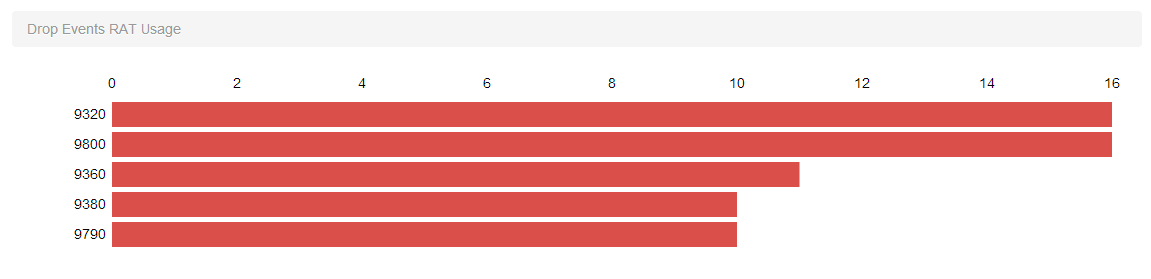
\includegraphics[scale=0.75]{chapter8/visualisation/bar_chart_1.png}
        \caption[Example Bar Chart output]
                {An Example Bar Chart output from the root node, highlighting all 
                 the various devices and their performance from a general point of 
                 view}
        \label{fig:bar_chart_1}
    \end{figure}
    ~\\
    \begin{figure}[H]
      \centering
        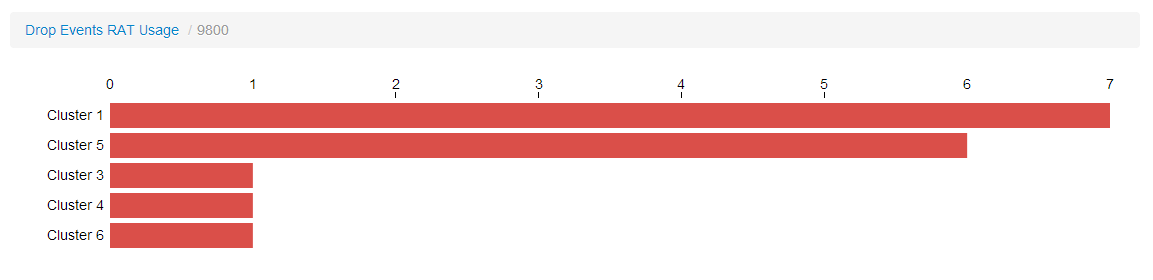
\includegraphics[scale=0.75]{chapter8/visualisation/bar_chart_2.png}
        \caption[Example Bar Chart output one node deep]
                {Example Bar Chart output one node deep --- i.e. all data that is
                 related to the 9800 device only.}
        \label{fig:bar_chart_2}
    \end{figure}
\end{landscape}


\newpage
\subsubsection{Circle Pack}
A Circle Pack diagram represents hierarchy through the use of embedded nodes. 
A Circle Pack diagram can be compared to a treemap, as it shares similar 
features however it is not as space-efficient. 

On the other hand it does reveal the overall size of each element (cluster, 
device, week, usage) more vividly in comparison to a treemap. Figure 
\ref{fig:circle_pack} illustrates an example output.

% Landscape page
\begin{landscape}
  % Center image
  \centering 
    \begin{figure}[H]
      \centering
        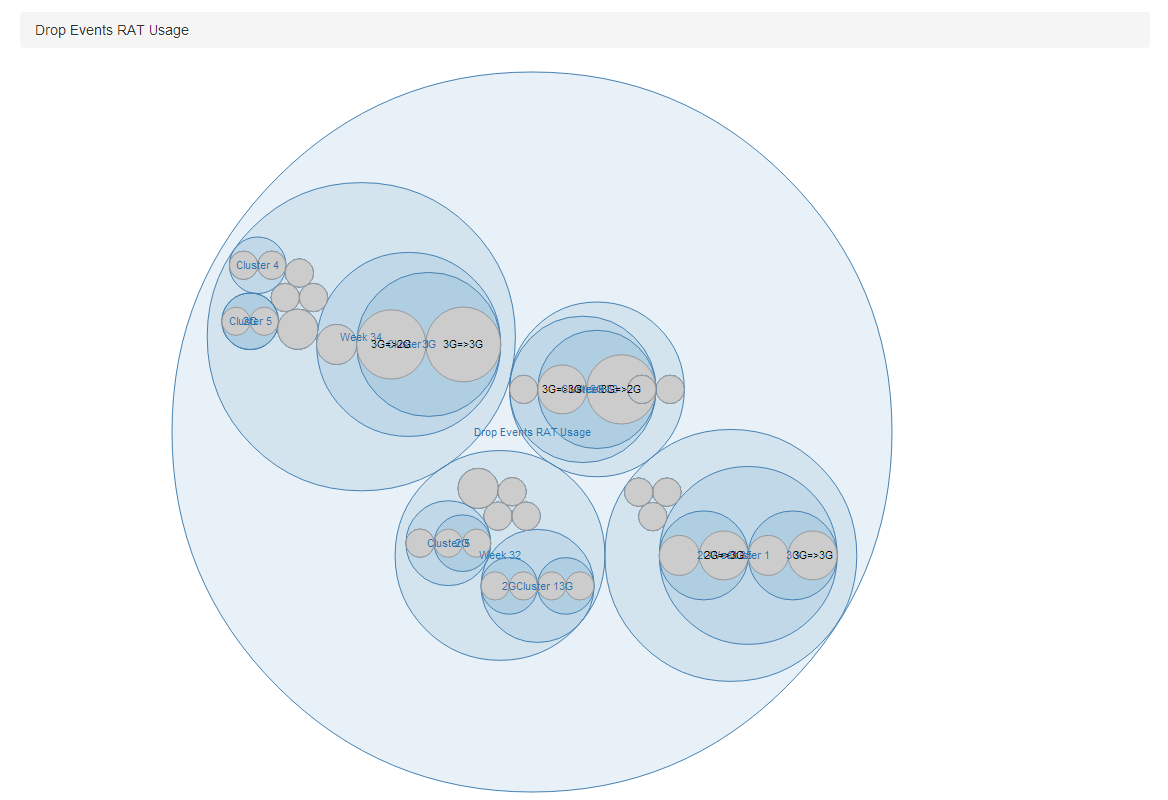
\includegraphics[scale=0.65]{chapter8/visualisation/circle_pack.png}
        \caption[Example Circle Pack output]
                {Example Circle Pack output, highlighting all the nodes. The 
               first node is the week, e.g. week 34.}
        \label{fig:circle_pack}
    \end{figure}
\end{landscape}


\newpage
\subsubsection{Dendrogram}

As with the Circle Pack diagram a dendrogram represents hierarchy through 
embedded nodes. A dendrogram is frequently used to illustrate the cluster 
arrangement formed by hierarchical clustering algorithms, although can be used 
in other ways.

Unlike the Circle Pack diagram, a dendrogram is not able to reveal the overall 
size of each element visually, and this has been shown via the raw value of 
events shown in brackets.

Figure \ref{fig:dendrogram} illustrates an example output.


% Landscape page
\begin{landscape}
  % Center image
  \centering 
    \begin{figure}[H]
      \centering
        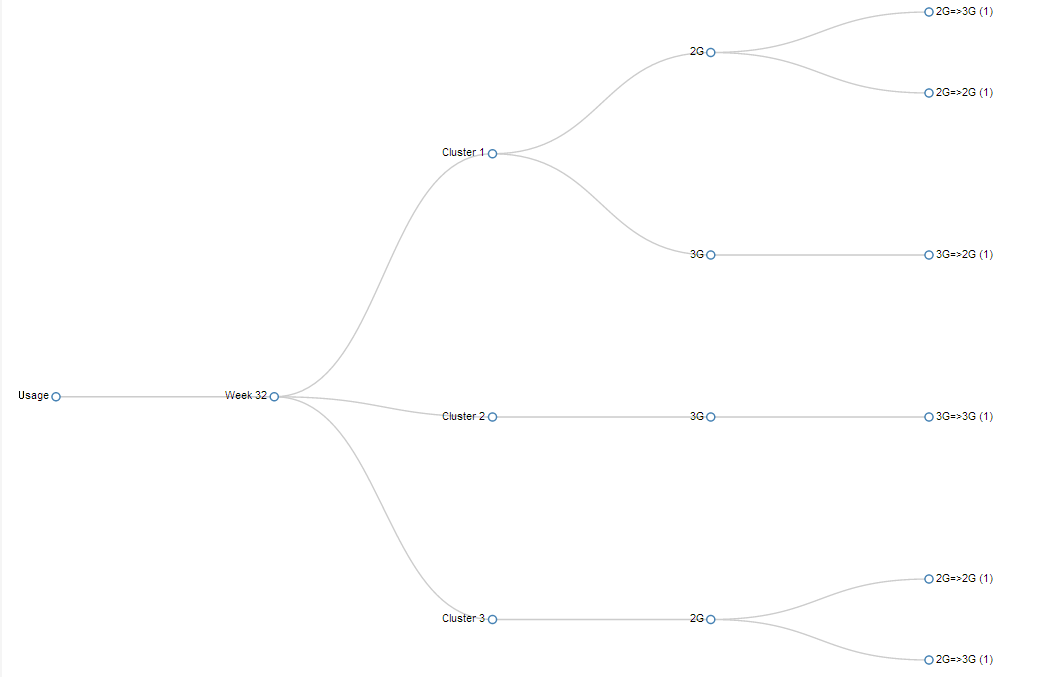
\includegraphics[scale=0.65]{chapter8/visualisation/dendrogram.png}
        \caption[Example Dendrogram output]
                {Example Dendrogram output, highlighting all the various for 
                the given week (week 32)}
        \label{fig:dendrogram}
    \end{figure}
\end{landscape}


\newpage
\subsubsection{Partition Chart}
A partition chart can thought of as an alternative to a pie chart. Although it 
looks more like a treemap, it more closely resembles the characteristics of a 
pie chart.

As with the previous charts, the partition chart supports hierarchical data. 
This allows the user to click upon a given area, and the chart will rearrange 
itself. This allows for a more bespoke, ``drilled down'' view to viewing the 
analysis.

Figure \ref{fig:partition_chart} highlights an example partition chart.

\begin{figure}[H]
  \centering
    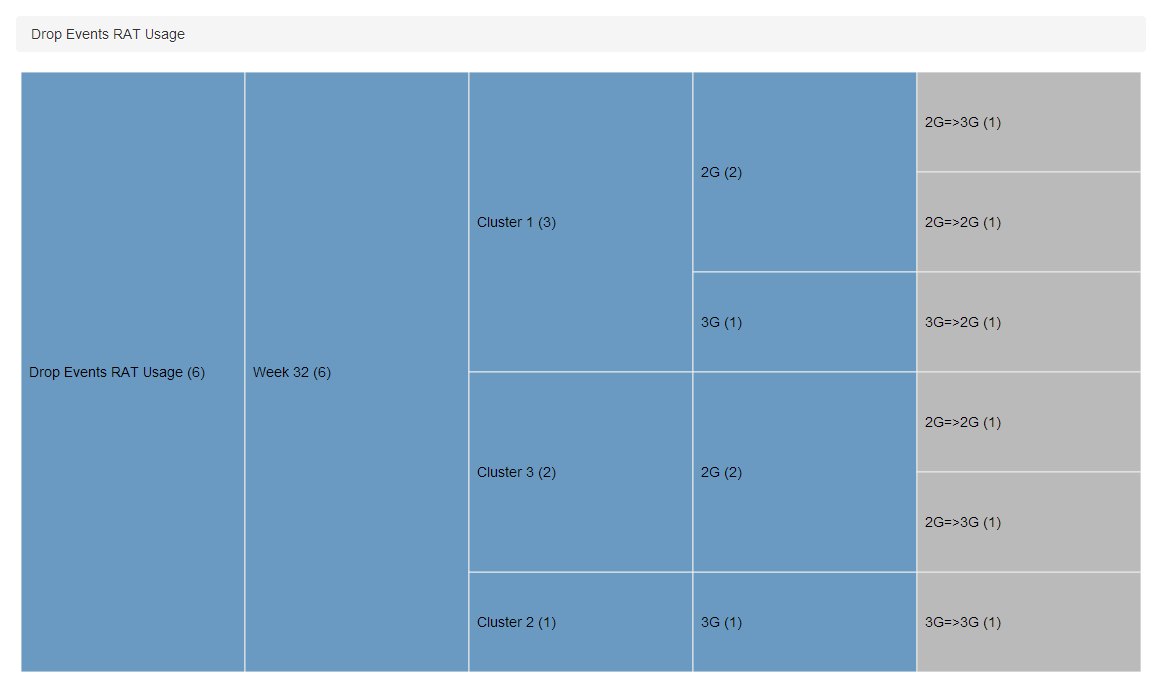
\includegraphics[scale=0.50]{chapter8/visualisation/partition.png}
    \caption[Example Partition output]
            {Example Partition output, highlighting all the nodes for the drop 
             events usage figures.}
    \label{fig:partition_chart}
\end{figure}


\newpage
\subsubsection{Treemap}
A treemap illustrates data as a set of nested rectangles. Like the partition 
chart, treemaps support hierarchical data structures.

Each square represents the total count of the events --- the larger the square 
the more events were found with the criteria. As with the partition chart, 
patterns within the data can be easily spotted. 

As a treemap grows, the efficiently of the use of space will also grow. The 
treemap implementation allows for a user to click upon a square, and it will 
rearrange itself, and as with many other charts will allow for a ``drilled 
down'' view.

Figure \ref{fig:treemap} highlights an example treemap.

\begin{figure}[H]
  \centering
    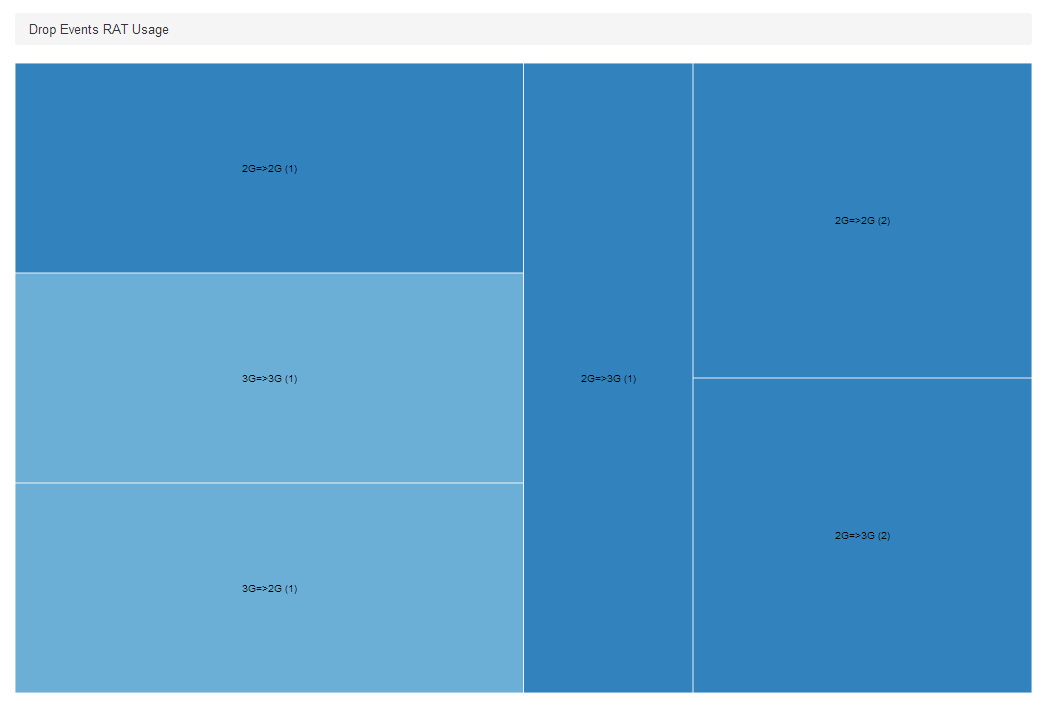
\includegraphics[scale=0.55]{chapter8/visualisation/treemap.png}
    \caption[Example Treemap output]
            {Example Treemap output, highlighting all the nodes for the drop 
             events usage figures.}
    \label{fig:treemap}
\end{figure}
